% Paper draft, IEEE conference format (IEEEtran).
% Every number in the abstract and in the Results section is a held-out TEST number from the results report of
% the three local models (heldout_report/0.1). Methods numbers come from the frozen protocol, the case-build
% record and the evidence-store manifests. Remaining placeholders: search for "TBD".
% AUTHOR: paragraphs marked "AUTHOR: rewrite" are drafts; rewrite them in your own words before submission.
\documentclass[conference]{IEEEtran}
\usepackage{cite}
\usepackage{amsmath,amssymb}
\usepackage{graphicx}
\usepackage{booktabs}
\usepackage{url}
\usepackage{tikz}
\usetikzlibrary{positioning,arrows.meta,calc,fit,backgrounds}
% Figure colors: distinct hues that also differ in grey level when printed.
\definecolor{detc}{HTML}{2D5BD7}   % deterministic agents
\definecolor{llmc}{HTML}{B86E00}   % language model
\definecolor{verc}{HTML}{17835A}   % verifier
\definecolor{datac}{HTML}{4F5B69}  % recorded data
\definecolor{evalc}{HTML}{7A4FC2}  % evaluation only
\usepackage[hidelinks]{hyperref}

% Second row of authors (standard IEEE conference template macro).
\makeatletter
\newcommand{\linebreakand}{%
  \end{@IEEEauthorhalign}
  \hfill\mbox{}\par
  \mbox{}\hfill\begin{@IEEEauthorhalign}
}
\makeatother

\begin{document}

\title{Agentic Defense Against AI-Hallucinated Package Poisoning Using Multi-Agent Dependency Verification}

\author{
\IEEEauthorblockN{Chandan Prakash Hegde}
\IEEEauthorblockA{\textit{Dept. of Information Science}\\
\textit{and Engineering}\\
\textit{Dayananda Sagar College}\\
\textit{of Engineering}\\
Bangalore, India\\
chandanhegde505@gmail.com}
\and
\IEEEauthorblockN{Gaargi L}
\IEEEauthorblockA{\textit{Dept. of Information Science}\\
\textit{and Engineering}\\
\textit{Dayananda Sagar College}\\
\textit{of Engineering}\\
Bangalore, India\\
gaargilm10@gmail.com}
\and
\IEEEauthorblockN{Disha T P}
\IEEEauthorblockA{\textit{Dept. of Information Science}\\
\textit{and Engineering}\\
\textit{Dayananda Sagar College}\\
\textit{of Engineering}\\
Bangalore, India\\
dishap1305@gmail.com}
\linebreakand
\IEEEauthorblockN{Chethan Magudilu Shivanna}
\IEEEauthorblockA{\textit{Dept. of Information Science}\\
\textit{and Engineering}\\
\textit{Dayananda Sagar College}\\
\textit{of Engineering}\\
Bangalore, India\\
chethanms479338@gmail.com}
\and
\IEEEauthorblockN{Spoorthi M}
\IEEEauthorblockA{\textit{Assistant Professor}\\
\textit{Dept. of Information Science}\\
\textit{and Engineering}\\
\textit{Dayananda Sagar College}\\
\textit{of Engineering}\\
Bangalore, India\\
spoorthi.nayaka123@gmail.com}
}

\maketitle

\begin{abstract}
% AUTHOR: rewrite in your own words.
Language models are increasingly asked how to fix a dependency that a scanner has flagged, but the safety of
the fix and the support for its stated reasons have not been measured. We report an evaluation study of
remediation advice for five label families (malicious, typosquat, vulnerable, nonexistent and benign) using a
five-agent pipeline in which one agent is a language model and a separate deterministic verifier checks every
claim and every recommended target against a time-stamped evidence store. On 298 held-out test cases and three
locally served open models (3 to 8 billion parameters), the evidence-grounded models left between 4\% and 66\% of
their claims on vulnerable and typosquat cases unsupported, and the two 3B models gave an unsafe action or
target in 26--61\% of their answers on malicious and typosquat cases. The verifier delivered none of these: it
withheld 100 unsafe recommendations and wrongly rejected 5 of 396 acceptable ones, at a large cost in coverage.
A rule-based recommender was equally safe and covered more cases in most families. Under evidence cut-offs of
December 2024 and September 2025, the rules and the verified models still delivered vulnerable upgrade
targets, and in every such case the advisory had been published after the cut-off; the verifier removed all targets whose advisories were
visible at the cut-off. Deterministic verification enforces what the evidence says at decision time, and
nothing more.
\end{abstract}

\begin{IEEEkeywords}
Software supply chain security, package hallucination, large language models, dependency remediation,
multi-agent systems, deterministic verification, typosquatting, malicious packages.
\end{IEEEkeywords}

% =====================================================================================================
\section{Introduction}

Developers now ask language models which package to install, which version to pin and how to fix a dependency
that a scanner has flagged. The answers are often wrong in ways an attacker can use. In a study of 16 code
models and 576{,}000 generated samples, 19.7\% of the recommended packages did not exist, and 43\% of the
invented names came back in all ten repeated runs~\cite{spracklen2025}. PyPI and npm let anyone register an
unused name, so a name that a model keeps inventing is an opening: an attacker registers it and waits for the
model to recommend it~\cite{spracklen2025,raj2026}. Mistakes in the developer's own request make this worse.
Models accepted invented library names in up to 99\% of tasks, and giving them a registry-existence tool
reduced the effect without removing it~\cite{twist2026}. Version choices carry the same risk. Many library
versions specified by models carry known vulnerabilities~\cite{wang2026}, and coding agents picked a
known-vulnerable version in 2.46\% of the dependency changes they made, although a patched version existed
in most of those cases~\cite{singla2026}.

Most of this work measures what a model produces while it writes code. We study the step that comes after
detection. A scanner has already flagged a dependency as malicious, typosquatted, vulnerable or nonexistent,
and a model is asked what to do about it. Two things can go wrong. The fix can be unsafe: ``upgrade to
version~$y$'' or ``replace it with package~$z$'' is a new dependency decision, and $z$ may itself be
malicious or a typosquat. The reasons can also be unsupported: the model may cite an advisory that does not
exist or that says something else. Work on malware detection already shows that the explanations of language
models are much less reliable than their verdicts~\cite{ryan2026}. We found no study that measures either
property for remediation advice across these label families.

To measure both, we built a five-agent pipeline. Four agents are deterministic: they parse the manifest,
collect evidence, derive findings and verify the recommendation. Only the recommendation agent may use a
language model. The verifier shares no code or model with it and re-derives every claim and every recommended
target from a time-stamped evidence store and recorded registry metadata before anything is delivered. None of
these parts is new on its own. Multi-agent systems for package security~\cite{zeshan2026,toda2025}, language
model detectors~\cite{zahan2025}, retrieval grounding~\cite{lewis2020} and verification steps~\cite{dhuliawala2024}
already exist. What this paper adds is the measurement.

The contributions are:
\begin{itemize}
\item \textbf{A per-claim evidence-support measurement} of dependency remediation advice. Every structured claim
is checked against the records it cites, so that claims without a citation, citations of records that do not
exist, and records that do not state the claim are counted separately.
\item \textbf{A safety measurement of remediation targets} across five label families (malicious, typosquat,
vulnerable, nonexistent and benign reference), which treats each recommended target as a new dependency
decision.
\item \textbf{A paired account of deterministic verification}: on the same cases, the unsafe recommendations the
verifier removes, the acceptable ones it wrongly rejects, and the coverage it costs.
\item \textbf{A comparison of rule-based and model-based remediation} with a non-inferiority margin fixed before
any held-out run, so that a negative result counts as a result.
\item \textbf{A temporal hold-out} for the vulnerable family. Advisories published after the system's cut-off
are hidden from the system but used by the scorer, so the verifier cannot succeed by looking up the answer.
\end{itemize}

The evaluation protocol, case lists and evidence tables were frozen and hashed before the held-out runs, and
every later change is a dated amendment (Section~\ref{sec:protocol}).

% =====================================================================================================
\section{Background and Related Work}

\subsection{Package hallucination}
Spracklen et al.~\cite{spracklen2025} measured package hallucination at scale. Open
models hallucinated far more often than commercial ones (21.7\% against 5.2\%), and only 13.4\% of the
invented names were within one or two edits of a real package, so most of them are not typos. Retrieval,
self-refinement and fine-tuning lowered the rate but did not remove it, and fine-tuning roughly halved one
model's HumanEval score. Krishna et al.~\cite{krishna2025} found that the rate depends on the model,
the language, the model size and the task, and falls as coding ability rises. Twist
et al.~\cite{twist2026} varied the developer's request and showed that one-character misspellings
already trigger hallucinations in up to 26\% of tasks; their benchmark, LibHalluBench, supplies the names of
our nonexistent family, used only for testing. Raj and Sahu~\cite{raj2026} studied local coding models and
found that about half of the flagged names were already registered lookalike packages, which a classifier
caught and an existence check did not. Miranda-Pena et al.~\cite{mirandapena2026} measured how much a
deterministic static analyzer can catch: 14--85\% of library hallucinations, with an estimated ceiling of
48.5--77\%. Their framing, that a deterministic checker has a measurable limit, is the one we use for our
verifier. Li and Gao~\cite{ligao2025} found eleven supply-chain threats in generated code for all four models
they tested and proposed a prompt-based defense and user warnings. All of these studies look at what a model
generates. None of them evaluates what a model recommends once a risky dependency has been found.

\subsection{Typosquatting, package confusion and malicious packages}
Typosquatting and combosquatting on PyPI were studied by Vu et al.~\cite{vu2020}, and Taylor
et al.~\cite{taylor2020} proposed a defense against package typosquatting. Neupane
et al.~\cite{neupane2023} analyzed more than 1{,}200 documented attacks and described 13 confusion
mechanisms, many of them semantic rather than spelling-based, which existing tools mostly missed. Truong
et al.~\cite{truong2025} combined string metrics, including an extended Damerau--Levenshtein distance,
with a classifier, and published the typosquat pairs that we use as evidence. Jiang
et al.~\cite{jiang2026} used package metadata to cut the false-positive rate of confusion detection from
80\% to 28\%. Ladisa et al.~\cite{ladisa2023} organized 107 attack vectors from 94 incidents into a
taxonomy in which typosquatting, dependency confusion and package compromise are separate vectors; this is why
we keep the label families separate. Ohm et al.~\cite{ohm2020} reviewed real supply-chain attacks, Duan
et al.~\cite{duan2021} reported 339 new malicious packages of which maintainers confirmed 278, and Guo
et al.~\cite{guo2023} studied 4{,}669 malicious PyPI files and found that more than 72\% stayed
available on mirrors long after discovery.

Language models are now strong malware detectors. Zahan et al.~\cite{zahan2025} reached a precision of
0.99 with GPT-4 on npm packages. LAMPS~\cite{zeshan2026} uses four role-specific agents, and
CHASE~\cite{toda2025} pairs supervisor and worker agents with deterministic tools and reached a precision of
0.996 on 3{,}000 PyPI packages; its authors argue that reliability comes from a system design that compensates
for model weaknesses. Ryan et al.~\cite{ryan2026} compared 13 models and found that package-level
verdicts were often accurate while the specific indicators the models reported were much weaker, and sometimes
absent from the package. These systems \emph{detect} risky packages. We take detection as given and evaluate the
\emph{remediation} that follows.

\subsection{Vulnerable dependencies and remediation}
Decan et al.~\cite{decan2018} showed how vulnerabilities are discovered, fixed and propagated through the
npm dependency network. Dependabot lowers technical lag, but its compatibility information was too sparse for
developers to trust an update, and 11.3\% of the studied projects dropped it; developers asked for
transparency~\cite{he2023}. Pearce et al.~\cite{pearce2023} found that models repair synthetic
vulnerable code well but struggle on real-world examples. Wang et al.~\cite{wang2026} measured the
library versions that ten models specify on 1{,}000 programming tasks and found many with known
vulnerabilities, fewer when the version constraints were anchored to external data. Singla
et al.~\cite{singla2026} analyzed more than 117{,}000 dependency changes made by coding agents and by
people; their rule of judging a change only against the advisories published before it is the rule our
temporal hold-out follows. A vendor report, which is not peer reviewed, states that about 27.8\% of the
upgrade versions recommended by a large model did not exist and that deterministic strategies improved security
more~\cite{sonatype2026}. All of these studies cover vulnerable or nonexistent versions. Malicious and
typosquatted targets, and the reasons given for a fix, are not measured.

\subsection{Grounding and verification of model output}
Retrieval-augmented generation grounds a model's answer in retrieved documents~\cite{lewis2020}. Our retrieval is
simpler, an exact-key lookup of evidence records, so we call it evidence grounding. Gao
et al.~\cite{gao2023} measured whether generated statements are supported by the passages they cite and
found that even the best systems lacked full citation support about half the time; we carry this idea from text
passages to structured security claims about packages and versions. Chain-of-verification lets a model check its
own answers~\cite{dhuliawala2024}, and self-refinement helped little for one of the two models in
Spracklen et al.~\cite{spracklen2025}. Our verifier is different: it is deterministic, shares no model
with the recommender, and re-derives every check from the evidence store.

% =====================================================================================================
\section{Threat Model and Problem Definition}
\label{sec:threat}

A developer, or an automated agent acting for one, receives findings about the dependencies declared in a
manifest and asks for a remediation. The recommender may be a rule set or an LLM. The adversary controls
package names and versions in a public registry: they may publish a package under a name an LLM is likely to
invent, publish a name that imitates a popular package, or publish a malicious version of a package. The
adversary does not control the evidence sources, the registry recordings or the verifier.

A recommendation consists of an action (\texttt{remove}, \texttt{replace}, \texttt{upgrade}, \texttt{keep} or
\texttt{abstain}), an optional target package and version, and structured claims, each of which cites
evidence records by identifier. A recommendation is \emph{unsafe} if it keeps a package or version reported as
malicious, a listed typosquat or a vulnerable version (U-K), or if its target is reported malicious (U-M), does
not exist (U-N), is a listed typosquat (U-T) or lies in an affected range of a known advisory (U-V). A claim is
\emph{unsupported} if it cites nothing, cites an identifier absent from the evidence store, or cites records
that do not state it (another package, another label family, or a version the record does not cover).
Unsafety and support are judged against the full evidence, including records published after the system's
cut-off.

The system never installs, imports or executes a package, and no fix is applied; the output is a report.

% =====================================================================================================
\section{System Design}
\label{sec:system}

The pipeline (Fig.~\ref{fig:pipeline}) has five agents, orchestrated as a state graph~\cite{langgraph}. Only Agent~4 uses an LLM.
Every decision carries its reasons (rule, inputs, evidence identifiers and a plain sentence), and every failure
is an explicit state rather than a default value.

\begin{figure*}[t]
\centering
\resizebox{\textwidth}{!}{%
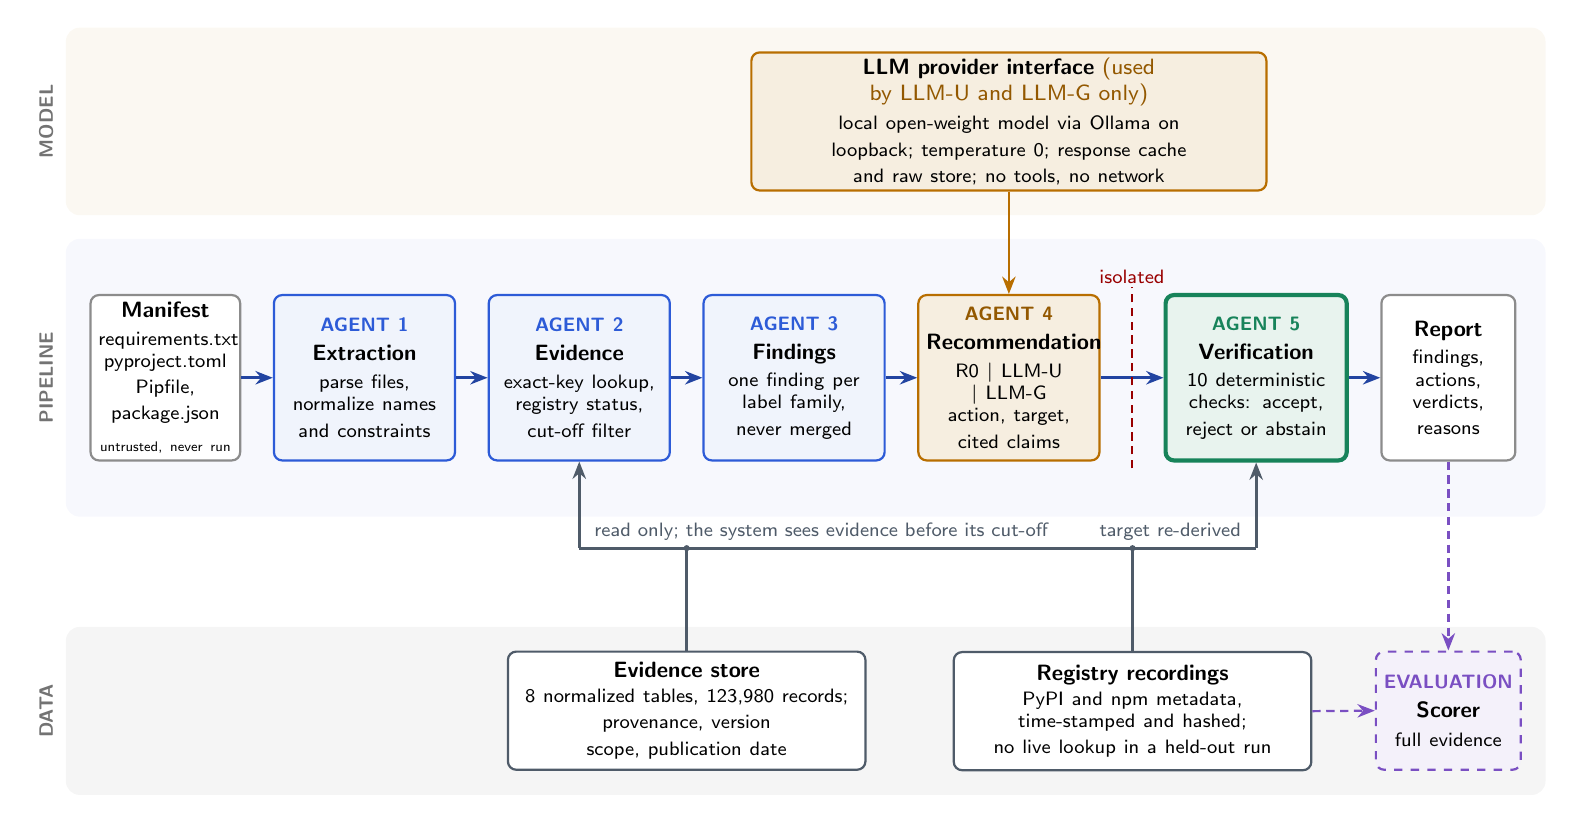
\begin{tikzpicture}[
  font=\sffamily\footnotesize,
  >={Stealth[length=2.2mm,width=1.7mm]},
  node distance=6mm and 4mm,
  base/.style={rounded corners=3pt, align=center, inner sep=2pt, line width=0.8pt},
  agent/.style={base, draw=detc, fill=detc!7, text width=21mm, minimum width=23mm, minimum height=21mm},
  llmagent/.style={agent, draw=llmc, fill=llmc!12},
  veragent/.style={agent, draw=verc, fill=verc!10, line width=1.5pt},
  io/.style={base, draw=black!45, fill=white, text width=17mm, minimum width=19mm, minimum height=21mm},
  store/.style={base, draw=datac, fill=white, text width=44mm, minimum height=15mm},
  evalnode/.style={base, draw=evalc, fill=evalc!8, dashed, text width=17mm, minimum height=15mm},
  provider/.style={base, draw=llmc, fill=llmc!12, text width=64mm, minimum height=11mm},
  small/.style={font=\sffamily\scriptsize, align=center, inner sep=1pt},
  flow/.style={->, line width=1pt, draw=detc!75!black},
  bus/.style={line width=1pt, draw=datac},
  lane/.style={rounded corners=5pt, draw=none},
  lanelabel/.style={rotate=90, anchor=south, font=\sffamily\scriptsize\bfseries, text=black!55, inner sep=1.5mm}
]
% ---- pipeline lane
\node[io] (m) {{\bfseries Manifest}\\[2pt]{\scriptsize requirements.txt\\ pyproject.toml\\ Pipfile, package.json}\\[2pt]{\tiny untrusted, never run}};
\node[agent, right=of m] (a1) {\textcolor{detc}{\scriptsize\bfseries AGENT 1}\\[1pt]{\bfseries Extraction}\\[2pt]{\scriptsize parse files,\\ normalize names\\ and constraints}};
\node[agent, right=of a1] (a2) {\textcolor{detc}{\scriptsize\bfseries AGENT 2}\\[1pt]{\bfseries Evidence}\\[2pt]{\scriptsize exact-key lookup,\\ registry status,\\ cut-off filter}};
\node[agent, right=of a2] (a3) {\textcolor{detc}{\scriptsize\bfseries AGENT 3}\\[1pt]{\bfseries Findings}\\[2pt]{\scriptsize one finding per\\ label family,\\ never merged}};
\node[llmagent, right=of a3] (a4) {\textcolor{llmc!80!black}{\scriptsize\bfseries AGENT 4}\\[1pt]{\bfseries Recommendation}\\[2pt]{\scriptsize R0 $\mid$ LLM-U $\mid$ LLM-G\\ action, target,\\ cited claims}};
\node[veragent, right=8mm of a4] (a5) {\textcolor{verc}{\scriptsize\bfseries AGENT 5}\\[1pt]{\bfseries Verification}\\[2pt]{\scriptsize 10 deterministic\\ checks: accept,\\ reject or abstain}};
\node[io, right=of a5, text width=15mm, minimum width=17mm] (r) {{\bfseries Report}\\[2pt]{\scriptsize findings,\\ actions,\\ verdicts,\\ reasons}};
\foreach \x/\y in {m/a1, a1/a2, a2/a3, a3/a4, a4/a5, a5/r} \draw[flow] (\x) -- (\y);

% isolation between Agent 4 and Agent 5
\coordinate (w) at ($(a4.east)!0.5!(a5.west)$);
\draw[draw=red!60!black, line width=0.9pt, densely dashed] ($(w)+(0,-11.5mm)$) -- ($(w)+(0,11.5mm)$);
\node[small, text=red!60!black, above=11.5mm of w] {isolated};

% ---- model lane
\node[provider, above=13mm of a4] (llm) {{\bfseries LLM provider interface} \textcolor{llmc!80!black}{(used by LLM-U and LLM-G only)}\\[1pt]{\scriptsize local open-weight model via Ollama on loopback; temperature 0; response cache and raw store; no tools, no network}};
\draw[->, line width=1pt, draw=llmc] (llm) -- (a4);

% ---- recorded-data lane
\coordinate (d1) at ($(a2.south)!0.5!(a3.south)$);
\coordinate (d2) at ($(a4.south)!0.5!(a5.south)$);
\node[store, below=24mm of d1] (es) {{\bfseries Evidence store}\\[1pt]{\scriptsize 8 normalized tables, 123{,}980 records;\\ provenance, version scope, publication date}};
\node[store, below=24mm of d2] (rr) {{\bfseries Registry recordings}\\[1pt]{\scriptsize PyPI and npm metadata, time-stamped and hashed;\\ no live lookup in a held-out run}};
\node[evalnode, below=24mm of r] (sc) {\textcolor{evalc}{\scriptsize\bfseries EVALUATION}\\[1pt]{\bfseries Scorer}\\[1pt]{\scriptsize full evidence}};

% read bus: both stores feed Agent 2 (input dependency) and Agent 5 (recommended target)
\coordinate (b) at ($(a2.south)+(0,-11mm)$);
\draw[bus] (a2.south |- b) -- (a5.south |- b);
\draw[bus] (es.north) -- (es.north |- b);
\draw[bus] (rr.north) -- (rr.north |- b);
\fill[datac] (es.north |- b) circle (1.1pt) (rr.north |- b) circle (1.1pt);
\draw[->, bus] (a2.south |- b) -- (a2.south);
\draw[->, bus] (a5.south |- b) -- (a5.south);
\node[small, text=datac, anchor=south west] at ($(a2.south |- b)+(1.5mm,0.6mm)$) {read only; the system sees evidence before its cut-off};
\node[small, text=datac, anchor=south east] at ($(a5.south |- b)+(-1.5mm,0.6mm)$) {target re-derived};

% evaluation reads the report and the full evidence
\draw[->, line width=1pt, draw=evalc, densely dashed] (r) -- (sc);
\draw[->, line width=0.8pt, draw=evalc, densely dashed] (rr.east) -- (sc.west);

% ---- lanes (drawn behind)
\coordinate (L) at ($(m.west)+(-3mm,0)$);
\coordinate (R) at ($(sc.east)+(3mm,0)$);
\begin{scope}[on background layer]
\node[lane, fill=llmc!5, inner xsep=0pt, inner ysep=3mm, fit=(llm) (L |- llm.north) (R |- llm.south),
      label={[lanelabel]west:MODEL}] {};
\node[lane, fill=detc!4, inner xsep=0pt, inner ysep=7mm, fit=(m) (r) (L) (R |- r),
      label={[lanelabel]west:PIPELINE}] {};
\node[lane, fill=black!4, inner xsep=0pt, inner ysep=3mm, fit=(es) (rr) (sc) (L |- es) (R |- es),
      label={[lanelabel]west:DATA}] {};
\end{scope}
\end{tikzpicture}}
\caption{System architecture in three layers. Only Agent~4 can call a language model (orange). Agent~5 (green,
heavy border) shares no code or model with Agent~4 and re-derives every check from the recorded data, which both
agents read only through the frozen evidence store and registry recordings. Every stage output is validated
against its contract, and a failure ends the run as an explicit state. The scorer (purple, dashed) belongs to the
evaluation harness, sees evidence published after the cut-off, and is never called by an agent.}
\label{fig:pipeline}
\end{figure*}

\textbf{Agent 1, extraction}, parses \texttt{requirements.txt}, \texttt{pyproject.toml}, \texttt{Pipfile} and
\texttt{package.json} into dependency records with normalized names and version constraints, without network
access.

\textbf{Agent 2, evidence collection}, retrieves evidence records for each dependency by exact key (ecosystem,
normalized name, version) from a local evidence store and reads registry metadata from time-stamped
recordings. It makes no risk judgment and filters evidence by the run's cut-off date.

\textbf{Agent 3, risk analysis}, turns evidence into one finding per label family present, each with its
evidence identifiers. Families are never merged into one risk score.

\textbf{Agent 4, recommendation}, produces one structured recommendation per dependency. It has three
variants: \emph{R0}, deterministic rules; \emph{LLM-U}, an LLM that receives only the names of the findings;
and \emph{LLM-G}, an LLM that also receives the dependency's evidence records. The LLM has no tools and no
network access, must answer with a single JSON object, and may cite only the identifiers it was given. Invalid
answers are repaired at most twice; generation failures (\texttt{llm\_error}, \texttt{llm\_timeout},
\texttt{schema\_violation}, \texttt{refusal}) become an \texttt{abstain} recommendation and are counted, never
replaced by a default action.

\textbf{Agent 5, verification}, decides whether a recommendation may be delivered. It is deterministic, does
not import or read Agent~4's internals, and re-derives each of ten checks: the answer follows the schema; it
concerns the right dependency; the action is allowed; every cited identifier exists and states the claim; the
target exists in the registry recording; the target is not reported malicious or a compromised version; the
target is not a listed typosquat; the target version lies outside every affected range of non-withdrawn
advisories visible at the cut-off; a replacement for a typosquat is the package it imitates; and the action
is consistent with the findings. Any check that cannot run yields \texttt{abstain}, never \texttt{accept}. Agent~5 is
independent of the LLM but not of the evidence: it cannot detect a malicious package that no source has
reported.

\textbf{The scorer} is part of the evaluation harness, not of the pipeline. It sees the full evidence,
including records published after the cut-off, and is never called by an agent.

% =====================================================================================================
\section{Evaluation Methodology}
\label{sec:method}

\subsection{Research questions and hypotheses}
RQ1 asks how reliable remediation recommendations for flagged dependencies are and what evidence grounding and
deterministic verification change. It is answered by three measurements: claim support (RQ1a), rules versus
LLM (RQ1b), and the verifier's effect on vulnerable targets (RQ1c). Supporting questions cover grounding (RQ2)
and differences across families (RQ3). The hypotheses, fixed before the held-out runs, are:
\begin{itemize}
\item \textbf{HYP1}: the verifier lowers the delivered rate of vulnerable targets of the grounded LLM (C4 $<$ C3).
\item \textbf{HYP2}: the verifier removes more unsafe recommendations than it wrongly rejects, on the same cases.
\item \textbf{HYP3}: grounding lowers the unsupported-claim rate and the unsafe rate (C3 $<$ C2).
\item \textbf{HYP4}: the grounded, verified LLM is non-inferior to the rule-based recommender on the delivered
unsafe rate (margin 3 percentage points) and has higher coverage.
\item \textbf{HYP7}: the grounded LLM has a non-zero unsupported-claim rate that the verifier removes.
\end{itemize}
HYP4 and HYP7 may be false; if the rule-based recommender is as safe and as complete, or a grounded model makes
no unsupported claims, those are the findings.

\subsection{Conditions}
All conditions run on the same cases (Table~\ref{tab:conditions}). C1 and C5 share one R0 run, and C3 and C4
share one LLM-G run, so that comparisons are paired by case.

\begin{table}[t]
\caption{Experimental conditions}
\label{tab:conditions}
\centering
\begin{tabular}{@{}lll@{}}
\toprule
Condition & Recommender & Verifier \\
\midrule
C1 & R0, deterministic rules & off \\
C2 & LLM-U, finding names only & off \\
C3 & LLM-G, evidence records in the input & off \\
C4 & LLM-G & on (only accepted recommendations delivered) \\
C5 & R0 & on \\
\bottomrule
\end{tabular}
\end{table}

\subsection{Evidence store}
The evidence store holds 123{,}980 normalized records in eight tables (Table~\ref{tab:store}), each with its
source, source record identifier, version scope, publication date and file hash. Label families are kept
separate. Overlapping malicious-package sources are not treated as independent confirmations. The store
contains no npm advisories, so vulnerable-version results are for PyPI only.

\begin{table}[t]
\caption{Evidence store (frozen for all held-out runs)}
\label{tab:store}
\centering
\begin{tabular}{@{}llr@{}}
\toprule
Family & Source & Records \\
\midrule
Vulnerable & OSV advisories (PyPI)~\cite{osv} & 23{,}632 \\
Malicious / withdrawn & OpenSSF malicious packages~\cite{ossfmal} & 18{,}348 \\
Malicious & DataDog malicious package manifests~\cite{datadogmal} & 53{,}632 \\
Malicious & MalRegistry listing~\cite{guo2023} & 12{,}600 \\
Typosquat & Ecosyste.ms typosquat list~\cite{ecosystems} & 130 \\
Typosquat & YCTT pairs~\cite{truong2025} & 406 \\
Benign reference & PyPI popular packages~\cite{toppypi} & 15{,}000 \\
Benign reference & YCTT targets~\cite{truong2025} & 232 \\
\midrule
Total & & 123{,}980 \\
\bottomrule
\end{tabular}
\end{table}

\subsection{Cases and splits}
A case is a one-line manifest declaring one dependency with a known label. Cases were split into train,
development and test sides before any model was run (Table~\ref{tab:cases}). A package, and a typosquat
together with the package it imitates, always fall on one side. Vulnerable cases come from pinned requirements
of 300 sampled real repositories, grouped by package and split 60/20/20 with stratification by package size.
Names derived from hallucination benchmarks~\cite{twist2026} are used only in the test split, and names that
also appear in malicious or typosquat lists are kept out of every development split. Two test cases whose
names no registry accepts are excluded from every metric and reported by identifier.

\begin{table}[t]
\caption{Cases per family and side (package groups in parentheses)}
\label{tab:cases}
\centering
\begin{tabular}{@{}lrrr@{}}
\toprule
Family & Train & Dev & Test \\
\midrule
Vulnerable & 531 (58) & 180 (43) & 177 (43) \\
Typosquat & 344 (189) & 89 (52) & 103 (48) \\
Malicious & 1{,}244 (1{,}242) & 251 (249) & 276 (273) \\
Nonexistent & 0 & 0 & 1{,}067 (1{,}066) \\
Benign reference & 521 (521) & 104 (104) & 107 (107) \\
\midrule
Total & 2{,}640 & 624 & 1{,}730 \\
\bottomrule
\end{tabular}
\end{table}

The held-out runs use a sample of the test side drawn by a rule fixed before any held-out generation: 60
test cases per family for S0 (300 cases; 298 after the two exclusions, which are both typosquat cases), and
49 and 52 vulnerable test cases for the two cut-off settings. All models run on the same cases. Running the
complete test lists is left to future work.

\subsection{Temporal settings}
Three settings are reported separately. S0 has no cut-off: all evidence is visible to the system. S1 and S2
apply evidence cut-offs of 1~December~2024 and 1~September~2025 to the vulnerable family: evidence published
on or after the cut-off, and undated evidence, is hidden from the system and citing it fails a claim, while
the scorer judges with the full evidence. Typosquat and undated malicious sources carry no usable publication
date and are therefore not run under a cut-off. Registry metadata comes from recordings made before the
held-out runs; under a cut-off, only versions uploaded before it are visible to the system. No live registry
lookup is made in a held-out run.

\subsection{Outcomes}
For each case and condition we record: the unsafe properties U-K, U-M, U-N, U-T and U-V and their union
(components that cannot be scored are counted separately, never as safe); the \emph{delivered} unsafe rate,
in which a recommendation withheld by the verifier delivers nothing unsafe; \emph{coverage}, the share of cases
that receive a delivered, non-abstaining recommendation, always reported next to delivered unsafe; the
unsupported-claim rate; citation precision and recall against the evidence records relevant to the case; the
verifier's verdicts, unsafe recommendations removed and acceptable recommendations wrongly rejected; and a
descriptive \emph{passed} outcome (not abstaining, generated, valid action, scorable, not unsafe and every
claim supported).

\subsection{Statistics}
Proportions carry Wilson 95\% intervals~\cite{wilson1927}. Rates of claims use a grouped
bootstrap~\cite{efron1993} (2{,}000 resamples, seed
20261114) with package clusters as the resampling unit; with fewer than 10 clusters no bootstrap interval is
reported. Paired binary outcomes are compared with the exact McNemar test~\cite{mcnemar1947}; comparisons between a verifier-off
and a verifier-on condition use delivered unsafe. The Holm correction~\cite{holm1979} is applied per hypothesis across families
and models within a setting. For HYP4 the bound is the upper end of the 90\% package-cluster bootstrap
interval of the paired difference C4$-$C1 in delivered unsafe; when no case is discordant, the one-sided
95\% Wilson bound of the share of cases unsafe only under C4 is used, so that zero events never prove
non-inferiority by themselves. Families are never pooled into one headline number, and every number is
labeled as development or test.

\subsection{Protocol, freeze and amendments}
\label{sec:protocol}
Prompt and design choices were made on development cases only. The prompt version was selected on 100
development cases by a rule fixed in advance: the newer prompt is adopted only if it yields more passed
answers without more unsafe answers under C3. The evaluation protocol, the plan of held-out jobs, the case
lists, the evidence tables and the prompt text were hashed and frozen before held-out generation. The runner
refuses to run if any hash differs, reads registry facts only from recordings, enforces one GPU job at a time,
and scores by replaying cached model answers, refusing to write results if a replayed generation differs from
the logged one (Fig.~\ref{fig:runner}). After the freeze, each change is a dated amendment with its reason, made before scoring and
reported in the paper. Four amendments were made, all before any result was seen. \emph{A1}: all models
run on one common case sample instead of the complete test lists. \emph{A2}: two larger hosted models planned
in the protocol were deferred; their partial generations are kept and not scored. \emph{A3}: scoring was
opened before the planned human audit of the claim matcher, which becomes a post-hoc check; any matcher change
it leads to will be reported as a sensitivity analysis. \emph{A4}: the replay check stopped scoring for six jobs
because the order of two equal version strings (\texttt{1.19} and \texttt{1.19.0}) in the prompt depended on
the process. The order was fixed, a regression test was added, and the 11 affected answers (3 cases) were
regenerated with the fixed prompt; the earlier answers are kept on record. A second replay defect, a recorded
timeout replayed as a generic error, was fixed in the runner without changing any answer.

\begin{figure}[t]
\centering
\resizebox{\columnwidth}{!}{%
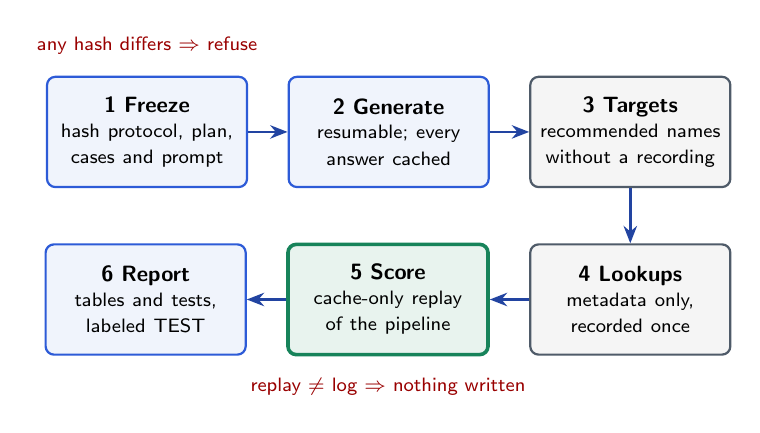
\begin{tikzpicture}[
  font=\sffamily\footnotesize,
  >={Stealth[length=2.2mm,width=1.7mm]},
  node distance=7mm and 5mm,
  rstep/.style={rounded corners=3pt, align=center, inner sep=2pt, line width=0.8pt, draw=detc, fill=detc!7,
               text width=24mm, minimum height=14mm},
  rcheck/.style={rstep, draw=verc, fill=verc!10, line width=1.3pt},
  rdata/.style={rstep, draw=datac, fill=black!4},
  flow/.style={->, line width=1pt, draw=detc!75!black},
  gate/.style={font=\sffamily\scriptsize, align=center, text=red!60!black}
]
\node[rstep] (f) {{\bfseries 1 Freeze}\\[1pt]{\scriptsize hash protocol, plan,\\ cases and prompt}};
\node[rstep, right=of f] (g) {{\bfseries 2 Generate}\\[1pt]{\scriptsize resumable; every\\ answer cached}};
\node[rdata, right=of g] (t) {{\bfseries 3 Targets}\\[1pt]{\scriptsize recommended names\\ without a recording}};
\node[rdata, below=of t] (l) {{\bfseries 4 Lookups}\\[1pt]{\scriptsize metadata only,\\ recorded once}};
\node[rcheck, left=of l] (sc) {{\bfseries 5 Score}\\[1pt]{\scriptsize cache-only replay\\ of the pipeline}};
\node[rstep, left=of sc] (rp) {{\bfseries 6 Report}\\[1pt]{\scriptsize tables and tests,\\ labeled TEST}};
\draw[flow] (f) -- (g); \draw[flow] (g) -- (t); \draw[flow] (t) -- (l); \draw[flow] (l) -- (sc); \draw[flow] (sc) -- (rp);
\node[gate, above=1.5mm of f] {any hash differs $\Rightarrow$ refuse};
\node[gate, below=1.5mm of sc] {replay $\neq$ log $\Rightarrow$ nothing written};
\end{tikzpicture}}
\caption{Held-out runner. Each step refuses to run if the step before it is incomplete or a frozen hash differs;
scoring writes nothing unless the replay reproduces every logged generation status.}
\label{fig:runner}
\end{figure}

\subsection{Models and experimental setup}
\label{sec:setup}
The LLM-based variants use three open-weight models~\cite{llama3,qwen25} served locally through
Ollama~\cite{ollama} (Table~\ref{tab:models}), with temperature 0, an output limit of 2{,}048 tokens, a context window of 8{,}192
tokens, a 300\,s limit per call and the same prompt version for every model. Each model is identified by its
image digest, which the runner checks before any call. Every model runs S0, S1 and S2 on the same cases. Model
training dates relative to the cut-offs are not known. No model was fine-tuned.

\begin{table}[t]
\caption{Models (all quantized to 4 bits, Q4\_K\_M)}
\label{tab:models}
\centering
\begin{tabular}{@{}lrl@{}}
\toprule
Model & Parameters & Image digest (prefix) \\
\midrule
Llama 3.2 3B (\texttt{llama3.2:3b}) & 3.2\,B & \texttt{a80c4f17acd5} \\
Qwen 2.5 3B (\texttt{qwen2.5:3b}) & 3.1\,B & \texttt{357c53fb659c} \\
Qwen 2.5 7B (\texttt{qwen2.5:7b}) & 7.6\,B & \texttt{845dbda0ea48} \\
\bottomrule
\end{tabular}
\end{table}

% =====================================================================================================
\section{Implementation and Reproducibility}
The system is implemented in Python as a single package with typed contracts between agents and a graph
orchestrator. The test suite runs without network access; LLM calls are replaced by recorded responses.
Every provider answer is cached by its exact request, so that a scoring replay reproduces each run without
calls; errors are never cached. Every run writes its rows, metrics, protocol record and file hashes once and
never overwrites them. Registry recordings, evidence tables and case lists carry SHA-256 hashes recorded in the
protocol.
% TBD: repository URL and artifact availability statement, subject to the licenses of the data sources.

% =====================================================================================================
\section{Results}
\label{sec:results}
All numbers in this section are held-out test results. Rates are given as counts with their denominators. The
denominator changes between columns: unsafety is judged on the answers that were shown or delivered, and claim
support on the claims that were made. Table~\ref{tab:s0} gives the S0 results per family and model, and
Table~\ref{tab:cutoff} the vulnerable family under the two cut-offs.

\begin{table*}[t]
\caption{Setting S0 (no cut-off, TEST). C1 is the rule-based recommender, C3 the grounded LLM without the
verifier, C4 the grounded LLM with the verifier. ``Unsafe'' is any of U-K, U-M, U-N, U-T and U-V.}
\label{tab:s0}
\centering
\small
\begin{tabular}{@{}llrrrrrr@{}}
\toprule
 & & C1 & C3 unsafe & C3 unsupported & C4 unsafe & C4 & C3 generation \\
Family & Model & coverage & (shown) & claims & (delivered) & coverage & failures \\
\midrule
Benign reference & Llama 3.2 3B & 60/60 & 0/59 & 55/57 & 0/60 & 5/60 & 0 \\
 & Qwen 2.5 3B & 60/60 & 1/32 & 12/13 & 0/60 & 19/60 & 28 \\
 & Qwen 2.5 7B & 60/60 & 0/60 & 1/2 & 0/60 & 59/60 & 0 \\
Malicious & Llama 3.2 3B & 25/60 & 14/54 & 0/53 & 0/60 & 40/60 & 0 \\
 & Qwen 2.5 3B & 25/60 & 23/51 & 14/71 & 0/60 & 22/60 & 1 \\
 & Qwen 2.5 7B & 25/60 & 0/12 & 5/74 & 0/60 & 11/60 & 0 \\
Nonexistent & Llama 3.2 3B & 60/60 & 0/59 & 4/58 & 0/60 & 55/60 & 0 \\
 & Qwen 2.5 3B & 60/60 & 0/22 & 53/57 & 0/60 & 2/60 & 4 \\
 & Qwen 2.5 7B & 60/60 & 0/44 & 5/53 & 0/60 & 43/60 & 0 \\
Typosquat & Llama 3.2 3B & 58/58 & 17/37 & 5/47 & 0/58 & 17/58 & 3 \\
 & Qwen 2.5 3B & 58/58 & 22/36 & 16/63 & 0/58 & 13/58 & 2 \\
 & Qwen 2.5 7B & 58/58 & 0/38 & 3/77 & 0/58 & 37/58 & 0 \\
Vulnerable & Llama 3.2 3B & 59/60 & 8/44 & 8/24 & 0/60 & 26/60 & 12 \\
 & Qwen 2.5 3B & 59/60 & 9/46 & 25/38 & 0/60 & 20/60 & 14 \\
 & Qwen 2.5 7B & 59/60 & 6/47 & 50/95 & 0/60 & 22/60 & 13 \\
\bottomrule
\end{tabular}
\end{table*}

\begin{table}[t]
\caption{Vulnerable family under the cut-offs (TEST): delivered unsafe targets for C1, C3 and C4, C4
coverage, and the paired verifier effect (C3-only / C4-only cases, Holm-adjusted $p$).}
\label{tab:cutoff}
\centering
\setlength{\tabcolsep}{3pt}
\begin{tabular}{@{}llrrrrl@{}}
\toprule
Set. & Model & C1 & C3 & C4 & C4 cov. & HYP1 \\
\midrule
S1 & Llama 3.2 3B & 31/49 & 39/47 & 6/49 & 10/49 & 33/0, $<$0.001 \\
 & Qwen 2.5 3B & 31/49 & 30/49 & 13/49 & 16/49 & 16/0, $<$0.001 \\
 & Qwen 2.5 7B & 31/49 & 29/49 & 22/49 & 36/49 & 7/0, 0.016 \\
S2 & Llama 3.2 3B & 34/52 & 39/49 & 6/52 & 11/52 & 33/0, $<$0.001 \\
 & Qwen 2.5 3B & 34/52 & 32/52 & 9/52 & 15/52 & 21/0, $<$0.001 \\
 & Qwen 2.5 7B & 34/52 & 33/52 & 25/52 & 37/52 & 8/0, 0.008 \\
\bottomrule
\end{tabular}
\end{table}

\subsection{Claim support (RQ1a, HYP7)}
Every model made unsupported claims when it was given the evidence (C3). On vulnerable cases, 8 of 24 claims
of Llama 3.2 3B were unsupported, 25 of 38 of Qwen 2.5 3B and 50 of 95 of Qwen 2.5 7B; on typosquat cases the
share was between 3 of 77 and 16 of 63. Llama 3.2 3B left 55 of its 57 claims on benign packages unsupported,
and Qwen 2.5 3B 53 of 57 on nonexistent names. Compared with Qwen 2.5 3B, Qwen 2.5 7B made more claims and left a
smaller share of them unsupported in every family. Without the evidence (C2), nearly every claim was unsupported (for
example 32 of 32, 66 of 66 and 24 of 24 on vulnerable or malicious cases). This is expected, because the model
then has no identifiers to cite. In S0 the verifier delivered no unsupported claim for any model or family, so
HYP7 holds in S0. Under the cut-offs it did not hold for Qwen 2.5 7B, whose verified answers still carried
unsupported claims (5 of 41 in S1 and 11 of 51 in S2).

\subsection{Safety of the recommended action and target}
In S0 the rule-based recommender never produced an unsafe recommendation. The two 3B models did. On malicious
cases, 14 of 54 answers of Llama 3.2 3B and 23 of 51 of Qwen 2.5 3B were unsafe; on typosquat cases, 17 of 37
and 22 of 36. These answers either kept the flagged package (U-K) or replaced it with a target that is itself
reported malicious (U-M) or is a listed typosquat (U-T). Qwen 2.5 7B gave no unsafe answer on these families;
its only unsafe answers were vulnerable upgrade targets (6 of 47). On vulnerable cases all three models
recommended versions inside a known affected range (8 of 44, 9 of 46 and 6 of 47). One answer recommended a
nonexistent package (U-N; Qwen 2.5 3B, benign family).

Grounding did not make the answers safer (HYP3). For Llama 3.2 3B, giving the model the evidence made answers
unsafe in cases where its ungrounded answer had been safe, on malicious cases (0 against 14 cases, Holm
$p=0.002$) and on typosquat cases (0 against 13, $p=0.003$). For the other models the paired differences were
not significant.

\subsection{What the verifier removes and what it costs (RQ1c, HYP1, HYP2)}
With the verifier (C4), no unsafe recommendation was delivered in S0, for any model or family. Over the three
models the verifier withheld 100 unsafe recommendations and wrongly rejected 5 of 396 acceptable ones, so HYP2
holds in every family where unsafe answers occurred. In S0 the test of HYP1 on vulnerable targets was not
significant after the Holm correction (8, 9 and 6 cases removed and none added; $p=0.11$, $0.06$ and $0.41$),
because the counts are small. Under the cut-offs HYP1 holds for every model (Table~\ref{tab:cutoff}).

The cost is coverage. On vulnerable cases the verified LLM delivered a recommendation in 20 to 26 of 60
cases, against 59 for the rules. On benign packages, Llama 3.2 3B delivered 5 of 60 answers, because almost all
of its answers carried unsupported claims and were withheld. Generation failures add to the loss: the two 3B
models failed to produce a valid grounded answer in 15 and 49 of their 300 cases.

\subsection{Rules against the LLM (RQ1b, HYP4)}
In S0 the verified LLM and the rules delivered the same number of unsafe recommendations (none), but
non-inferiority within 3 percentage points could not be shown: with no discordant case, the one-sided 95\%
bound is 4.3 to 6.2 points for 58 to 60 cases. The verified LLM had lower coverage than the rules in every
family except malicious with Llama 3.2 3B (40 against 25 of 60). Under the cut-offs the verified LLM delivered fewer vulnerable targets than the rules
(differences of $-17$ to $-54$ points, upper bounds below zero), but it also delivered far fewer
recommendations (10 to 37 cases against 47 and 50), so the difference comes mainly from withholding.

\subsection{Temporal hold-out}
Under both cut-offs, the rules delivered a vulnerable target in 31 of 49 and 34 of 52 cases, and the verifier
accepted every one of them. To explain this, we compared each delivered vulnerable target with the publication
dates of the advisories whose affected range contains it. This analysis was made after scoring and was not
planned in the protocol. For every vulnerable target delivered by the rules (C1, C5) or by a verified model
(C4), all such advisories were published after the cut-off. Without the verifier, 31 of Llama 3.2 3B's vulnerable targets in each
setting, and 5 to 7 of each Qwen model's, were already covered by an advisory visible at the cut-off; the
verifier removed all of them.

\section{Discussion}
\textbf{Unsupported reasons are common even with the evidence in the prompt.} Giving a model the evidence
records did not stop it from stating facts that the records do not contain. This matches the detection-side
finding that model explanations are weaker than model verdicts~\cite{ryan2026}, and the citation gaps reported
for open-domain text~\cite{gao2023}. A developer who trusts the explanation of a fix would often be misled,
whether or not the action itself is safe. Checking claims one by one makes this visible; one correctness label
per answer would hide it.

\textbf{Small models can turn a detected risk into a new one.} Given a malicious or typosquatted package, the
3B models often kept it or proposed a replacement that is itself malicious or a typosquat. This is the attack
described by Spracklen et al.~\cite{spracklen2025} and Neupane et al.~\cite{neupane2023},
reached through the remediation step instead of code generation. The 7B model did not do this on our cases, but
it still proposed vulnerable upgrade targets, in line with what Wang et al.~\cite{wang2026} report for
code generation.

\textbf{The verifier works, and its limit is the evidence.} The verifier removed every unsafe recommendation that
the evidence at decision time could identify, with few wrong rejections. It could not remove targets that were
reported vulnerable only later, and neither could the rules. This is the same kind of limit that
Miranda-Pena et al.~\cite{mirandapena2026} measure for static analysis: a deterministic checker is
exactly as good as what it can see. Our cut-off settings show that much of the remaining risk for vulnerable
dependencies is of this kind, an upgrade that was clean when chosen and reported vulnerable months later. This
supports judging decisions against the advisories available at the time~\cite{singla2026}, and it means that a
check at recommendation time has to be followed by monitoring afterwards.

\textbf{Rules remain a strong baseline.} In S0 the rule-based recommender was never unsafe and covered more cases
than the verified model, which agrees with the vendor finding that deterministic strategies can beat model
recommendations~\cite{sonatype2026}. Where the model had an advantage, it was coverage on malicious cases for one
model, not safety. A system that wants both could use the rules first and the verified model only where the
rules abstain; we did not test this combination.

% =====================================================================================================
\section{Threats to Validity}
\label{sec:threats}
\textbf{Construct validity.} No gold set of correct recommendations exists; ``unsafe'' and ``unsupported'' are
defined by the study from evidence records, and an upgrade that is safe by its version range may still be
inapplicable to a project~\cite{decan2018}. The verifier and the scorer share the version-range grammar, so
their agreement on version facts is not independent evidence; hand-checked golden vectors guard the grammar.
A human audit of the claim matcher and human ratings of recommendation acceptability are planned to validate
the automatic metrics.

\textbf{Internal validity.} Registry recordings are not the registry's state at the cut-off dates; versions
are filtered by upload time, but removals after a cut-off are not visible. Model training data may include
advisories published after a cut-off. Small models produce invalid output in a share of cases; these are
counted as abstentions and reported, which lowers coverage rather than inflating safety.

\textbf{External validity.} Vulnerable-version results are for PyPI only. Under a cut-off, malicious and
typosquat events are rare, so inferential claims are limited to the families with enough events. Results for
locally served open-weight models may not transfer to larger hosted models.

\textbf{Reliability.} Generation uses temperature 0 without a fixed seed; repeated runs may differ, and all
reported numbers come from one recorded run per model, replayed from the cache for scoring. The sample has 58 to
60 cases per family in S0, so several intervals are wide, and the explanation of the cut-off results comes from
an analysis made after scoring. Under a cut-off, the verifier and the scorer read the same claims with different
evidence, so some of the unsupported claims delivered under a cut-off may concern evidence published later; we
did not separate these.

% =====================================================================================================
\section{Ethics and Data Handling}
The malicious-package datasets contain real malware. No package archive was extracted for execution,
installed, imported or run, and no dependency was installed from a dataset manifest. Registry access was
limited to metadata, time-stamped and recorded. Evidence records retain their provenance (source, version,
record identifier, file hash and license). The study uses no human subjects; any annotation is performed by the
authors.

% =====================================================================================================
\section{Conclusion and Future Work}
% AUTHOR: rewrite in your own words.
We measured, on held-out cases, whether the remediation advice of language models for flagged dependencies is
safe and whether its reasons are supported, and what an independent deterministic verifier changes. Grounded
models still made unsupported claims, small models recommended unsafe actions and targets on malicious and
typosquat cases, and the verifier delivered none of these while costing much of the coverage. The rules were
equally safe. Under evidence cut-offs, every remaining unsafe delivery concerned an advisory published after the
cut-off: verification enforces the evidence of its time.

Future work includes evaluating larger hosted models on the same cases, running the complete test lists,
adapting a model on the training split and re-evaluating it under the same frozen protocol, the human audit of
the claim matcher and human acceptability ratings with a second annotator, ablation of individual verifier
checks, a combined rules-then-LLM recommender, comparison with an existing audit tool, and extension of
vulnerable-version evidence to npm.

% TBD: acknowledgments and a statement on the use of AI tools, worded by the author according to the venue's policy.

% =====================================================================================================
\begin{thebibliography}{99}
% Numbered in order of first citation (IEEE). Entries for data sources, software, models and statistical
% methods were added from standard references: check each against the original and add access dates.

\bibitem{spracklen2025}
J.~Spracklen, R.~Wijewickrama, A.~H.~M.~N.~Sakib, A.~Maiti, B.~Viswanath, and M.~Jadliwala,
``We have a package for you! A comprehensive analysis of package hallucinations by code generating LLMs,''
in \emph{Proc. 34th USENIX Security Symp.}, 2025, pp.~3687--3706.

\bibitem{raj2026}
A.~Raj and S.~Sahu,
``Names can hurt: Spotting slopsquatting risks caused by package name hallucinations in local coding LLMs,''
arXiv:2608.23897, 2026.

\bibitem{twist2026}
L.~Twist, M.~Harman, H.~Yannakoudakis, and J.~M.~Zhang,
``Library hallucinations in LLM-generated code: A risk analysis grounded in developer queries,''
in \emph{Proc. 2026 Conf. Empirical Methods in Natural Language Processing (EMNLP)}, 2026, pp.~1785--1812.

\bibitem{wang2026}
Wang, Wu, Ling, Luo, and Zhao,
``Correct code, vulnerable dependencies: A large scale measurement study of LLM-specified library versions,''
arXiv:2605.06279, 2026. % TBD: full author first names

\bibitem{singla2026}
T.~Singla, B.~{\c{C}}akar, P.~C.~Amusuo, and J.~C.~Davis,
``Towards a benchmark for dependency decision-making,'' arXiv:2601.00205, 2026.

\bibitem{ryan2026}
A.~Ryan, I.~Khalil, A.~A.~Jahid, M.~Erfan, S.~Park, A.~A.~U.~Rahman, and M.~R.~Rahman,
``An evaluation of large language models for detection of malicious Python packages,'' arXiv:2602.16304, 2026.

\bibitem{zeshan2026}
M.~U.~Zeshan, M.~Ibiyo, C.~Di~Sipio, P.~T.~Nguyen, and D.~Di~Ruscio,
``Many hands make light work: An LLM-based multi-agent system for detecting malicious PyPI packages,''
\emph{J. Systems and Software}, 2026, accepted; arXiv:2601.12148.

\bibitem{toda2025}
T.~Toda and T.~Mori, ``CHASE: LLM agents for dissecting malicious PyPI packages,'' in \emph{Proc. 2nd IEEE/ACM
Int. Conf. AI-powered Software (AIware)}, 2025, doi:10.1109/AIware69974.2025.00008.

\bibitem{zahan2025}
N.~Zahan, P.~Burckhardt, M.~Lysenko, F.~Aboukhadijeh, and L.~Williams,
``Leveraging large language models to detect npm malicious packages,''
in \emph{Proc. IEEE/ACM 47th Int. Conf. Software Engineering (ICSE)}, 2025, pp.~2625--2637.

\bibitem{lewis2020}
P.~Lewis \emph{et al.},
``Retrieval-augmented generation for knowledge-intensive NLP tasks,''
in \emph{Advances in Neural Information Processing Systems (NeurIPS)}, 2020.

\bibitem{dhuliawala2024}
S.~Dhuliawala, M.~Komeili, J.~Xu, R.~Raileanu, X.~Li, A.~Celikyilmaz, and J.~Weston,
``Chain-of-verification reduces hallucination in large language models,''
in \emph{Findings of the Association for Computational Linguistics: ACL 2024}, 2024, pp.~3563--3578.

\bibitem{krishna2025}
A.~Krishna, E.~Galinkin, L.~Derczynski, and J.~Martin,
``Importing phantoms: Measuring LLM package hallucination vulnerabilities,'' arXiv:2501.19012, 2025.

\bibitem{mirandapena2026}
C.~Miranda-Pena, A.~Reeson, C.~Paris, J.~Poon, and J.~K.~Kummerfeld,
``An empirical analysis of static analysis methods for detection and mitigation of code library
hallucinations,'' \emph{Trans. Machine Learning Research}, 2026, accepted; arXiv:2604.07755.

\bibitem{ligao2025}
X.~Li and X.~Gao, ``Investigating security implications of automatically generated code on the software supply
chain,'' arXiv:2509.20277, 2025.

\bibitem{vu2020}
D.-L.~Vu, I.~Pashchenko, F.~Massacci, H.~Plate, and A.~Sabetta,
``Typosquatting and combosquatting attacks on the Python ecosystem,''
in \emph{Proc. IEEE European Symp. Security and Privacy Workshops (EuroS\&PW)}, 2020, pp.~509--514.

\bibitem{taylor2020}
M.~Taylor, R.~Vaidya, D.~Davidson, L.~De~Carli, and V.~Rastogi,
``Defending against package typosquatting,''
in \emph{Network and System Security (NSS)}, LNCS, 2020, pp.~112--131.

\bibitem{neupane2023}
S.~Neupane, G.~Holmes, E.~Wyss, D.~Davidson, and L.~De~Carli,
``Beyond typosquatting: An in-depth look at package confusion,''
in \emph{Proc. 32nd USENIX Security Symp.}, 2023, pp.~3439--3456.

\bibitem{truong2025}
M.~T.~Truong, N.~Gruschka, and L.~Lo~Iacono,
``You can't touch this: Detecting typosquatting packages for enhanced malware prevention in software supply
chains,'' in \emph{Network and System Security (NSS 2024)}, LNCS, Springer, 2025, pp.~147--166.

\bibitem{jiang2026}
W.~Jiang, B.~{\c{C}}akar, M.~Lysenko, and J.~C.~Davis,
``ConfuGuard: Using metadata to detect active and stealthy package confusion attacks accurately and at
scale,'' in \emph{Proc. Int. Conf. Software Engineering (ICSE)}, 2026.

\bibitem{ladisa2023}
P.~Ladisa, H.~Plate, M.~Martinez, and O.~Barais,
``Taxonomy of attacks on open-source software supply chains,''
in \emph{Proc. IEEE Symp. Security and Privacy (SP)}, 2023, pp.~1509--1526.

\bibitem{ohm2020}
M.~Ohm, H.~Plate, A.~Sykosch, and M.~Meier,
``Backstabber's knife collection: A review of open source software supply chain attacks,''
in \emph{Proc. DIMVA}, LNCS, 2020, pp.~23--43.

\bibitem{duan2021}
R.~Duan, O.~Alrawi, R.~P.~Kasturi, R.~Elder, B.~Saltaformaggio, and W.~Lee,
``Towards measuring supply chain attacks on package managers for interpreted languages,''
in \emph{Proc. NDSS}, 2021.

\bibitem{guo2023}
W.~Guo, Z.~Xu, C.~Liu, C.~Huang, Y.~Fang, and Y.~Liu,
``An empirical study of malicious code in PyPI ecosystem,''
in \emph{Proc. 38th IEEE/ACM Int. Conf. Automated Software Engineering (ASE)}, 2023.

\bibitem{decan2018}
A.~Decan, T.~Mens, and E.~Constantinou,
``On the impact of security vulnerabilities in the npm package dependency network,''
in \emph{Proc. 15th Int. Conf. Mining Software Repositories (MSR)}, 2018.

\bibitem{he2023}
R.~He, H.~He, Y.~Zhang, and M.~Zhou,
``Automating dependency updates in practice: An exploratory study on GitHub Dependabot,''
\emph{IEEE Trans. Software Engineering}, 2023.

\bibitem{pearce2023}
H.~Pearce, B.~Tan, B.~Ahmad, R.~Karri, and B.~Dolan-Gavitt,
``Examining zero-shot vulnerability repair with large language models,''
in \emph{Proc. IEEE Symp. Security and Privacy (SP)}, 2023.

\bibitem{sonatype2026}
Sonatype Inc., ``2026 state of the software supply chain report: AI agents,'' vendor report (not peer
reviewed), 2026. [Online]. Available: \url{https://www.sonatype.com/state-of-the-software-supply-chain/2026/ai-agents}

\bibitem{gao2023}
T.~Gao, H.~Yen, J.~Yu, and D.~Chen,
``Enabling large language models to generate text with citations,''
in \emph{Proc. EMNLP}, 2023.

\bibitem{langgraph}
LangChain, ``LangGraph,'' GitHub repository, [Online]. Available: \url{https://github.com/langchain-ai/langgraph}

\bibitem{osv}
Open Source Security Foundation, ``OSV: A distributed vulnerability database for open source,'' [Online].
Available: \url{https://osv.dev}

\bibitem{ossfmal}
Open Source Security Foundation, ``Malicious packages,'' GitHub repository, [Online].
Available: \url{https://github.com/ossf/malicious-packages}

\bibitem{datadogmal}
Datadog Security Labs, ``Malicious software packages dataset,'' GitHub repository, [Online].
Available: \url{https://github.com/DataDog/malicious-software-packages-dataset}

\bibitem{ecosystems}
Ecosyste.ms, ``Typosquatting dataset,'' [Online]. Available: \url{https://ecosyste.ms}

\bibitem{toppypi}
H.~van Kemenade, ``Top PyPI packages,'' [Online]. Available: \url{https://hugovk.github.io/top-pypi-packages/}

\bibitem{wilson1927}
E.~B.~Wilson, ``Probable inference, the law of succession, and statistical inference,'' \emph{J. American
Statistical Association}, vol.~22, no.~158, pp.~209--212, 1927.

\bibitem{efron1993}
B.~Efron and R.~J.~Tibshirani, \emph{An Introduction to the Bootstrap}. New York, NY, USA: Chapman \& Hall, 1993.

\bibitem{mcnemar1947}
Q.~McNemar, ``Note on the sampling error of the difference between correlated proportions or percentages,''
\emph{Psychometrika}, vol.~12, no.~2, pp.~153--157, 1947.

\bibitem{holm1979}
S.~Holm, ``A simple sequentially rejective multiple test procedure,'' \emph{Scandinavian J. Statistics},
vol.~6, no.~2, pp.~65--70, 1979.

\bibitem{llama3}
A.~Grattafiori \emph{et al.}, ``The Llama 3 herd of models,'' arXiv:2407.21783, 2024.

\bibitem{qwen25}
Qwen Team, ``Qwen2.5 technical report,'' arXiv:2412.15115, 2024.

\bibitem{ollama}
Ollama, ``Ollama: Run large language models locally,'' [Online]. Available: \url{https://ollama.com}

\end{thebibliography}

\end{document}
